\documentclass[reqno,onecolumn,letterpaper,12pt]{article}
\usepackage[margin=1in]{geometry}
\usepackage{longtable}
\usepackage{bm}
\PassOptionsToPackage{hyphens}{url}\usepackage{hyperref}
\hypersetup{
    colorlinks=true,
    linkcolor=black,
    filecolor=black,
    urlcolor=black,
    citecolor=black
}
\usepackage{graphicx}
\usepackage{soul}
\usepackage{rotating}
\usepackage{amsmath}
\usepackage{setspace}
\usepackage{amssymb}
\usepackage{longtable}
\usepackage[longnamesfirst,sort]{natbib}
\usepackage{lscape}
\usepackage{amsfonts}
\usepackage[table]{xcolor}
\usepackage{booktabs}
\usepackage{subcaption}
\usepackage{courier}

\newcommand\citeapos[1]{\citeauthor{#1}'s (\citeyear{#1})}
\newcommand{\R}{\texttt{R}} % Write R in typewriter font

\begin{document}

%\title{{\bf Appendix for:} \\Complex Dependence in Foreign Direct Investment: \\Network Theory and Empirical Analysis} %\footnote{This work was supported by NSF grants SES-1558661, SES-1619644,
% SES-1637089, CISE-1320219, SMA-1360104, and IGERT Grant DGE-1144860. Any opinions, findings, and conclusions or recommendations are those of the authors and
% do not necessarily reflect those of the sponsor.}}
%\author{John  Schoeneman\thanks{\footnotesize{
%jbs5686@psu.edu, PhD Student, Pennsylvania State University.}} \and Boliang Zhu\thanks{\footnotesize{bxz14@psu.edu, Assistant Professor, Department of Political
%Science, Pennsylvania State University. }} \and Bruce A. Desmarais\thanks{\footnotesize{
%bdesmarais@psu.edu, Associate Professor, Department of Political Science, Pennsylvania State University.}}}
%\date{}
%\maketitle

%\thispagestyle{empty}
%\singlespacing
%\begin{abstract}
%    \noindent We develop theory that accounts for complex dependence in foreign direct investment (FDI) relationships. Conventional theories of FDI focus on firm-, industry-, country-, or dyad-level characteristics to account for cross-border capital movements. Yet, today's globalization is characterized by the increasing fragmentation and dispersion of production processes, which gives rise to complex dependence among production relationships. Consequently, FDI flows should be represented and theorized as a network. Specifically, we argue that FDI flows are reciprocal and transitive. We test these hypotheses along with conventional covariate determinants of FDI using an exponential random graph model (ERGM) for weighted networks. We find that FDI networks exhibit strong reciprocity and transitivity. Our network approach to studying FDI provides new insights into global investment flows and their political and economic consequences, and more generally the dynamics of globalization. In addition to our substantive findings, we offer a broad methodological contribution by introducing the ERGM for count-weighted networks in political science. %(150 words)


    %We study the structure of the international network of foreign direct investment (FDI). Existing studies based on regression models overlook the complex dependencies that are likely to characterize the FDI network. Recent developments in methodology for studying international relations show that regression is inadequate for quantitatively modeling dyadic data. We integrate hypotheses regarding exogenous covariate determinants and structural network dependencies into an exponential random graph model (ERGM) for weighted networks. We find that the FDI network exhibits both reciprocity and transitivity. These dependencies have been omitted from previous empirical models, which has consequences for inferences regarding covariate effects. In addition to our substantive findings, we offer a broad methodological contribution by introducing the ERGM for count-weighted networks in political science.

%\end{abstract}
%~\\

%{\bf Pre-submission to-do}
%\begin{itemize}
%\item \st{reduce abstract to 125 words}
%\item \st{Do a general read through for grammar}
%\item \st{Why don't we pool? With dyadic data we can identify effects. See significant heterogeneity. Beginning in 2008 we see a shift. This may be
%    attributable to the great recession.}
%\item Figures re-ordered and made into long table
%\item Discussion of Pooled Plots
%\item \st{footnote 12: justify use of Stock as DV}
%\item \st{Correlation table in appendix.}
%\item \st{Total outward FDI}

%\end{itemize}

\clearpage
\doublespacing
\setcounter{page}{1}
\renewcommand{\thesection}{Appendix \Alph{section}}
\renewcommand\thetable{\Alph{table}}
\renewcommand\thefigure{\Alph{figure}}
\appendix

\begin{centering}
\section*{Appendix}
\end{centering}

\section{Summary Statistics}\label{sum_stats}


\begin{table}[ht]
\caption{Correlation Matrix}
\label{cor_mat}
\centering
\begin{tabular}{rlllllllllll}
\\[-1.8ex]\hline
\hline \\[-1.8ex]
 & Distance & Defense Treaty & Polity & Trade Openness  \\ 
  \hline
  Distance & 1 &  &  &  \\ 
  Defense Treaty & -0.39**** & 1  &  &   \\ 
  Polity &  0.01**** &  0.06**** & 1 &   \\ 
  Trade Openness & -0.06**** & -0.04**** & -0.07**** & 1   \\ 
  PTA Depth & -0.41**** &  0.19**** &  0.18**** &  0.06****   \\ 
  BIT  & -0.08**** &  0.01**** &  0.02**** &  0.03****   \\ 
  Mass &  0.00     &  0.07**** &  0.10**** & -0.17****   \\ 
  Alliance Treaty & -0.35**** &  0.85**** &  0.07**** & -0.04****  \\ 
 GDP pc & -0.08**** &  0.04**** &  0.16**** &  0.24****   \\ 
  Trade Volume & -0.22**** &  0.18**** &  0.23**** & -0.06****  \\ 
  OECD pair & -0.23**** &  0.28**** &  0.20**** &  0.01**** \\ 
\hline \\[-1.8ex]
\\[-1.8ex]\hline
\hline \\[-1.8ex]

 &  PTA Depth & BIT & Mass & Alliance  Treaty  \\ 
  \hline
  PTA Depth &  1 &  &  &    \\ 
  BIT  & 0.07**** &1  &  &    \\ 
  Mass &   0.10**** &  0.14**** &1  &    \\ 
  Alliance Treaty  &  0.17**** &  0.02**** &  0.14**** & 1  \\ 
 GDP pc &  0.15**** &  0.09**** &  0.40**** &  0.10****  \\ 
  Trade Volume  &  0.28**** &  0.14**** &  0.72**** &  0.22****   \\ 
  OECD pair  &  0.31**** & -0.01**** &  0.29**** &  0.29****  \\ 
\hline \\[-1.8ex]
\\[-1.8ex]\hline
\hline \\[-1.8ex]

 & GDP pc & Trade Volume & OECD pair \\ 
  \hline
 GDP pc & 1 &  &\\ 
  Trade Volume &  0.34**** & 1 &\\ 
  OECD pair  &  0.23**** &  0.34****&1 \\ 
\hline \\[-1.8ex]
\\[-1.8ex]\hline
\hline \\[-1.8ex]

\end{tabular}
\end{table}

\clearpage

\begin{longtable}{c@{\hskip -.8cm}c}
\caption{\label{fig:sum_stats} Frequency count bar-plots for binary variables and distribution plots for continuous variables.}\\

Alliance Treaty &Defense Treaty\\ 
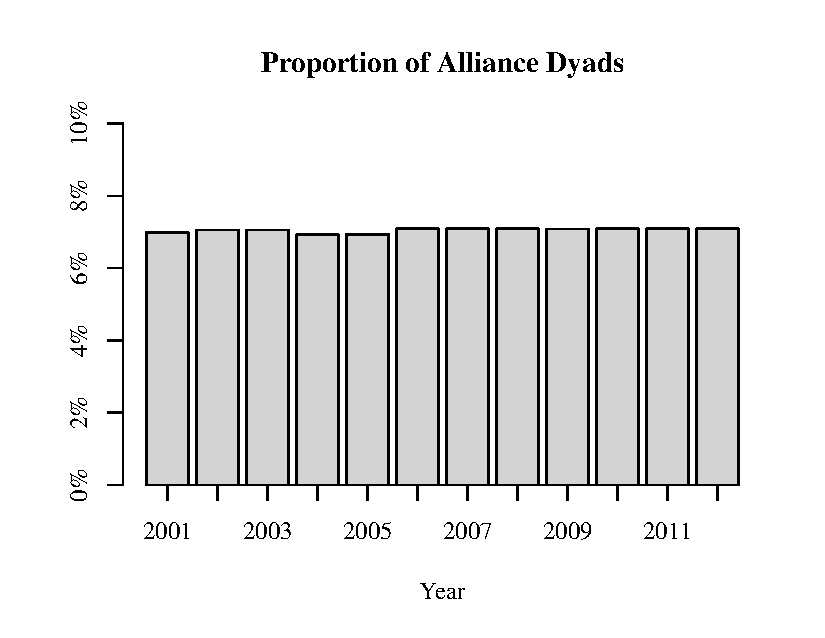
\includegraphics[height=.17\textheight, clip=true, trim=0cm 1cm 0cm 2cm]{SI_figures/descriptive_plots/alliance_barplot.pdf}    &
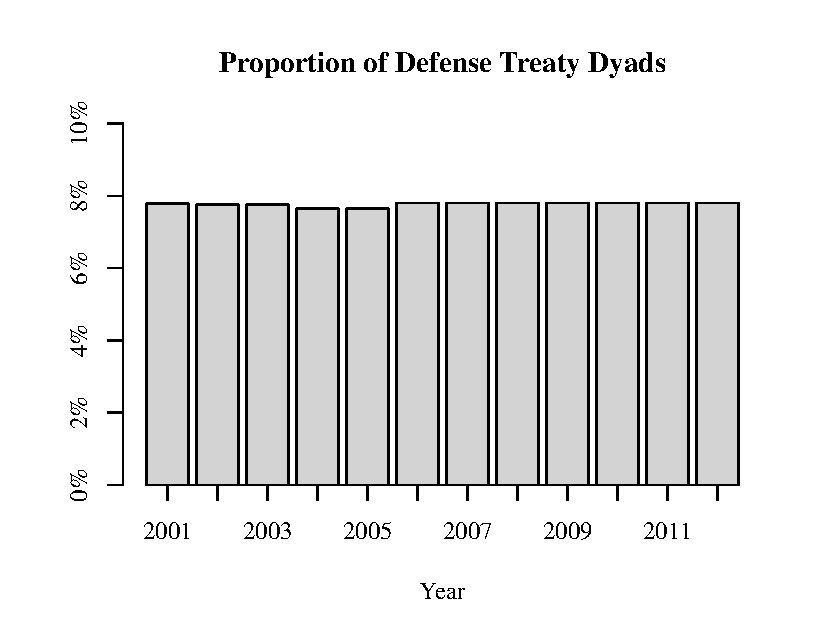
\includegraphics[height=.17\textheight, clip=true, trim=0cm 1cm 0cm 2cm]{SI_figures/descriptive_plots/defense_barplot.pdf}   \\

Bilateral Investment Treaty& OECD Pairs \\
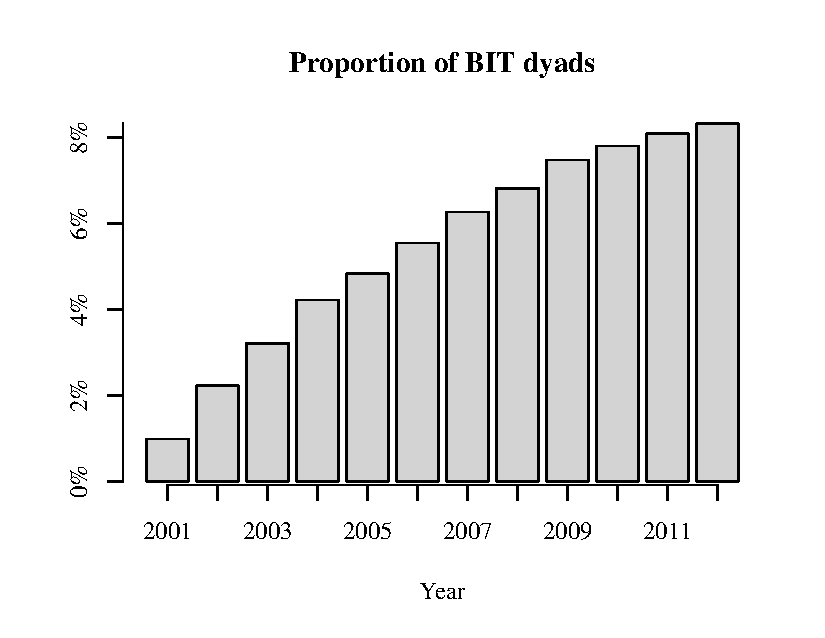
\includegraphics[height=.17\textheight, clip=true, trim=0cm 1cm 0cm 2cm]{SI_figures/descriptive_plots/BIT_barplot.pdf} &
 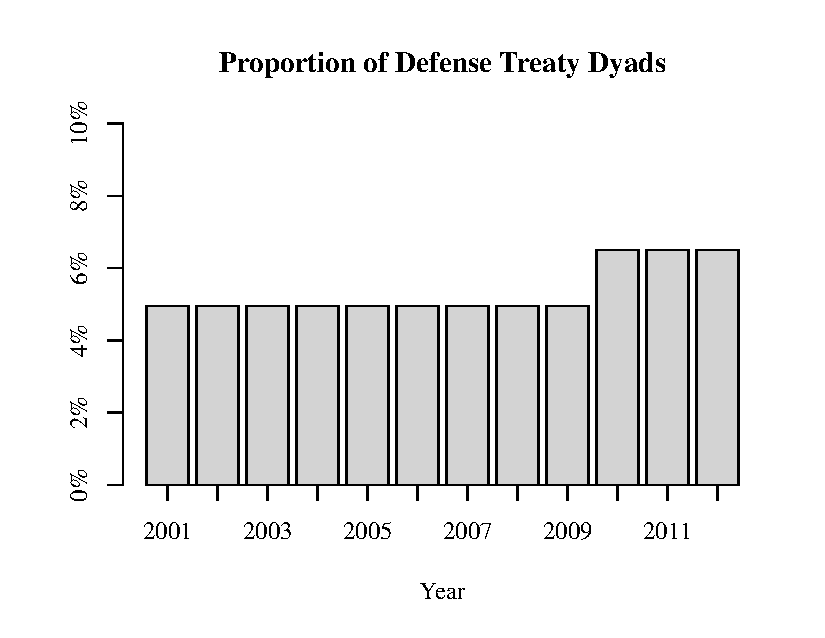
\includegraphics[height=.17\textheight, clip=true, trim=0cm 1cm 0cm 2cm]{SI_figures/descriptive_plots/OECDpair_barplot.pdf} \\

Dyad GDP Product &Distance\\
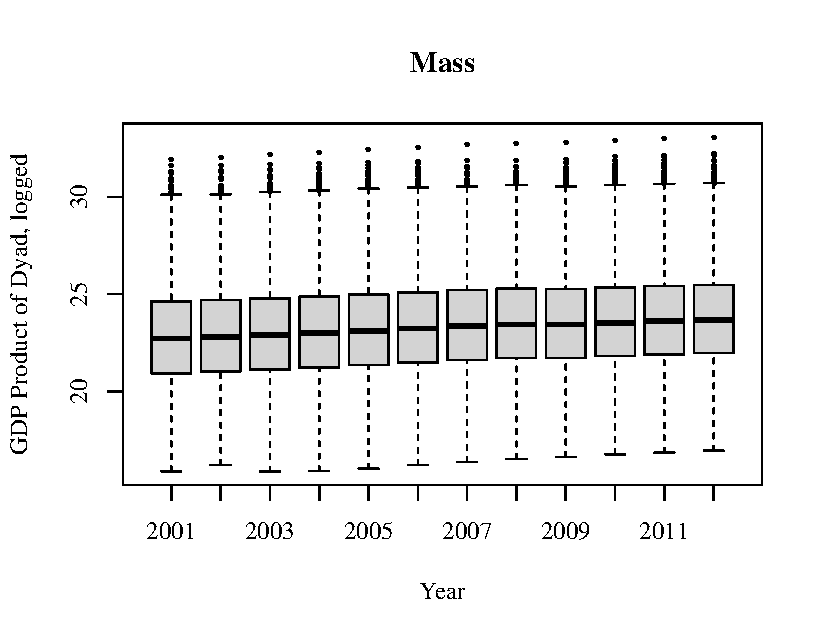
\includegraphics[height=.17\textheight, clip=true, trim=0cm 1cm 0cm 2cm]{SI_figures/descriptive_plots/Mass_boxplot.pdf}    &
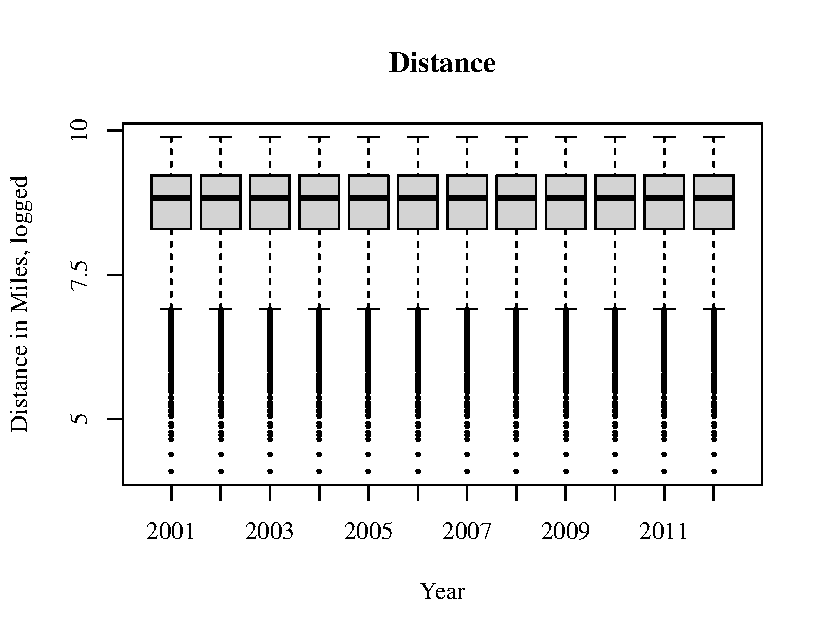
\includegraphics[height=.17\textheight, clip=true, trim=0cm 1cm 0cm 2cm]{SI_figures/descriptive_plots/dist_boxplot.pdf}   \\

GDP per capita & Polity\\
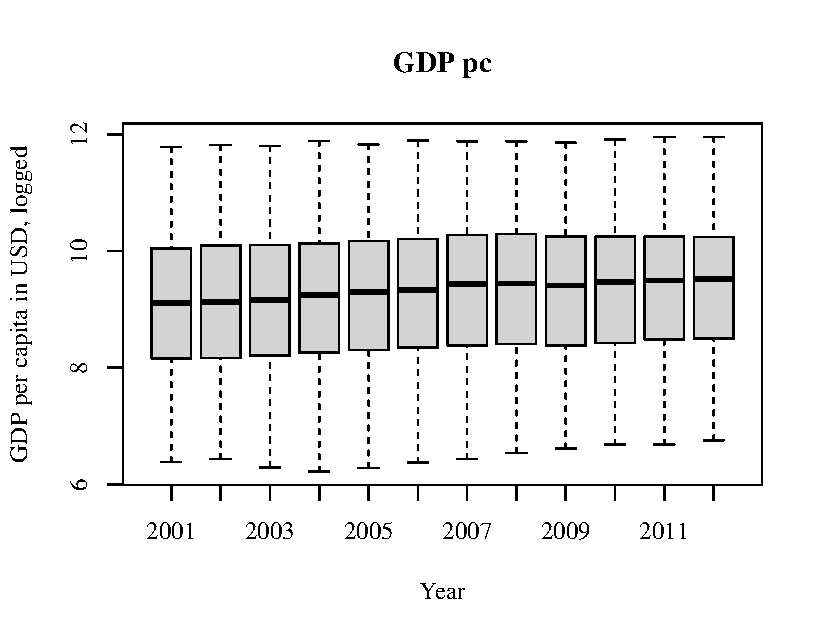
\includegraphics[height=.17\textheight, clip=true, trim=0cm 1cm 0cm 2cm]{SI_figures/descriptive_plots/GDPpc_boxplot.pdf}    &
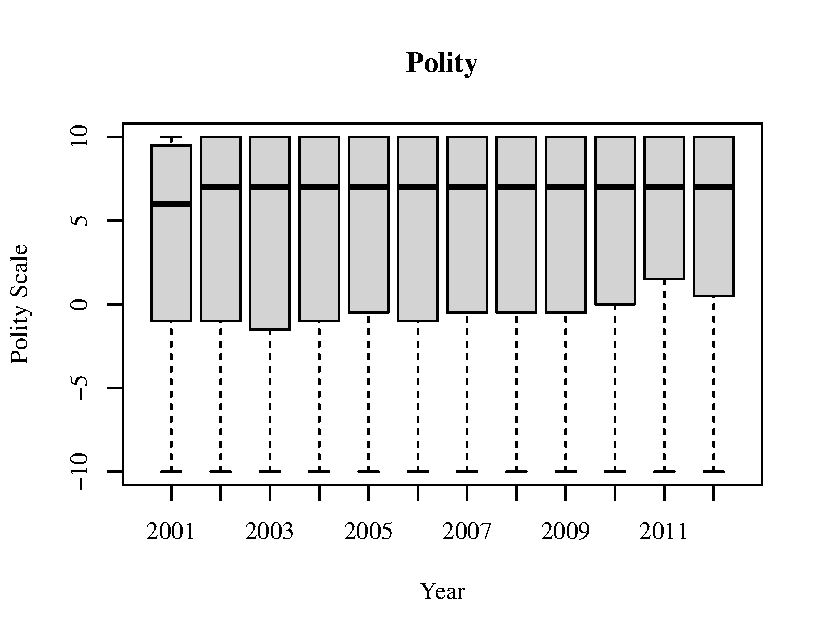
\includegraphics[height=.17\textheight, clip=true, trim=0cm 1cm 0cm 2cm]{SI_figures/descriptive_plots/polity_boxplot.pdf}  \\

\clearpage

Trade as \% of GDP &
Trade Volume\\
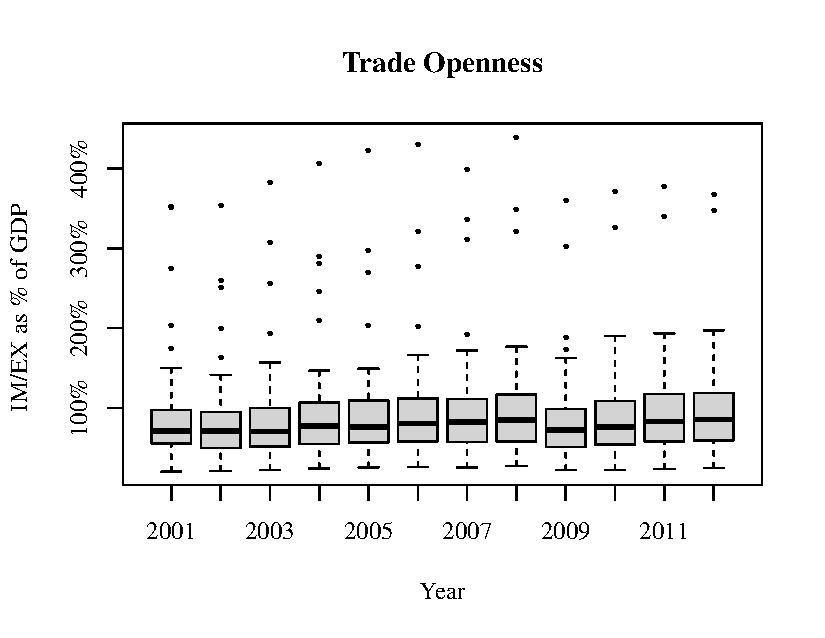
\includegraphics[height=.17\textheight, clip=true, trim=0cm 1cm 0cm 2cm]{SI_figures/descriptive_plots/TO_boxplot.pdf}   &
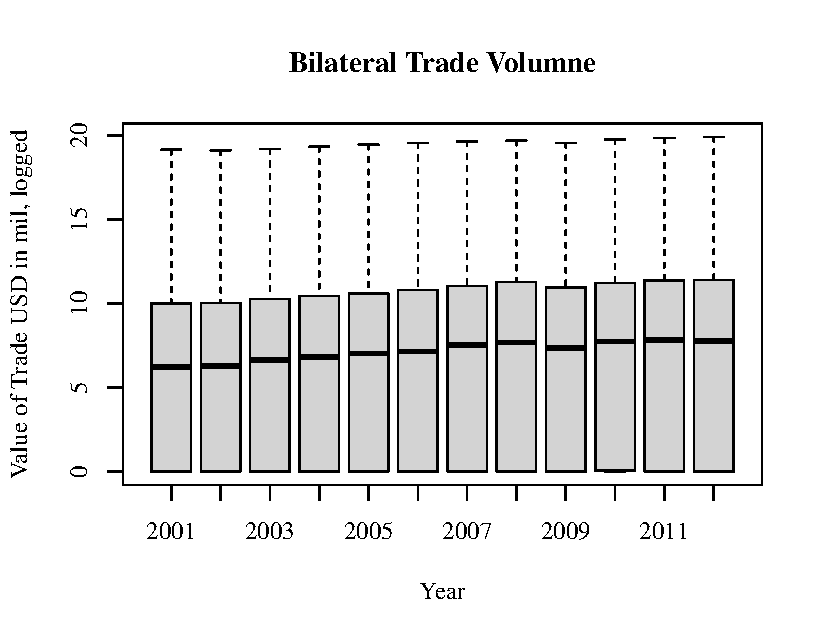
\includegraphics[height=.17\textheight, clip=true, trim=0cm 1cm 0cm 2cm]{SI_figures/descriptive_plots/Trade_boxplot.pdf}   \\

PTA Depth & FDI Stock\\
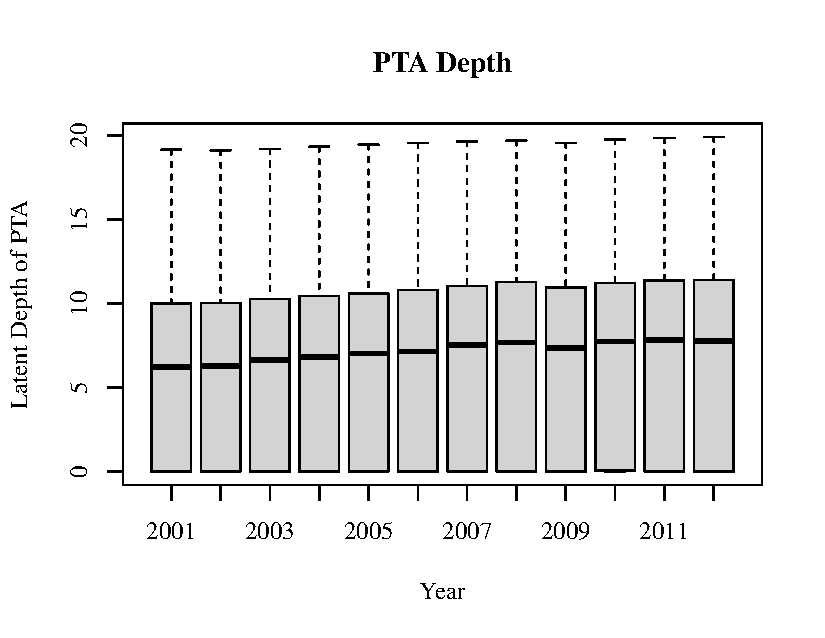
\includegraphics[height=.17\textheight, clip=true, trim=0cm 1cm 0cm 2cm]{SI_figures/descriptive_plots/ptadepth_boxplot.pdf} &
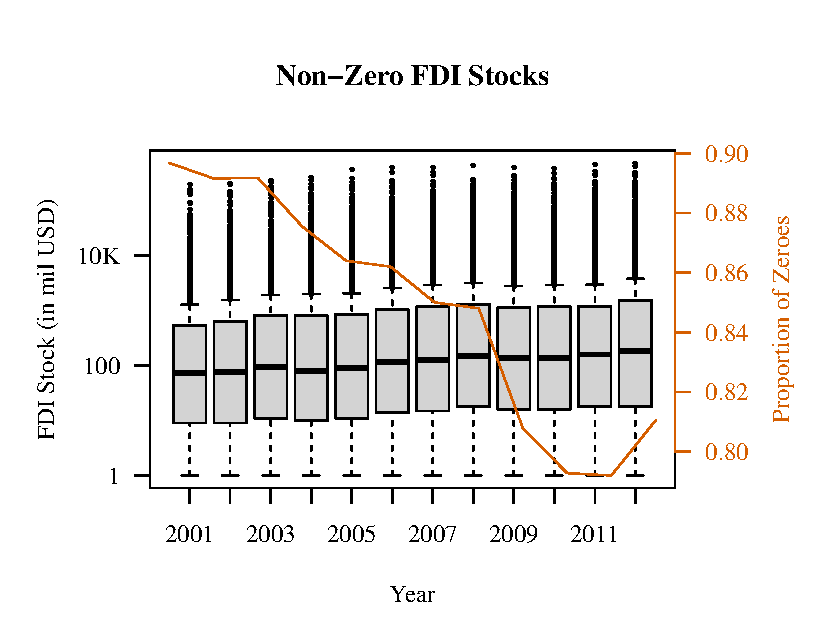
\includegraphics[height=.17\textheight, clip=true, trim=0cm 1cm 0cm 2cm]{SI_figures/descriptive_plots/fdi_stock_zeroes_boxplot.pdf}  \\


\end{longtable}




\begin{figure}[!h]
\centering
Bilateral and World FDI stocks\\
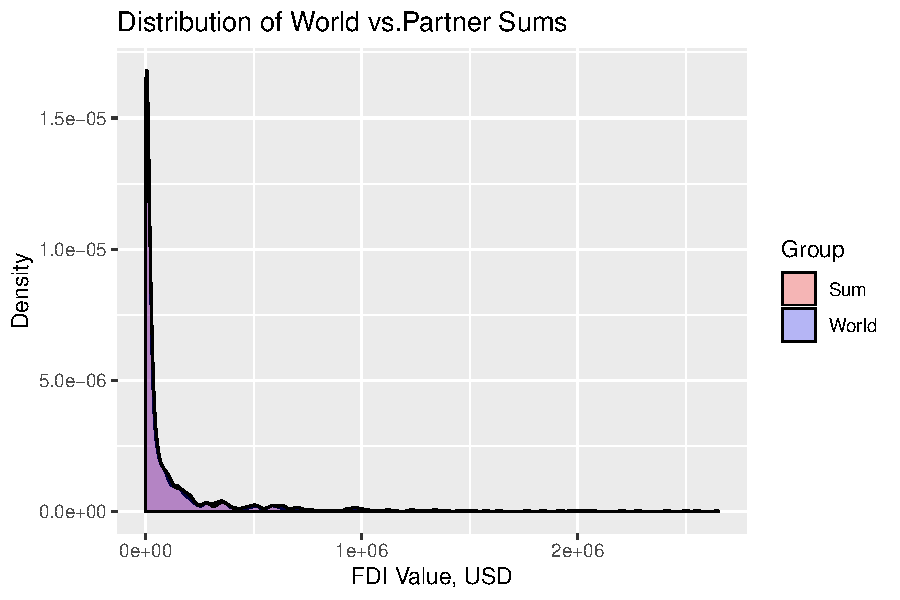
\includegraphics[height=.4\textheight, clip=true, trim=0cm 0cm 0cm .6cm]{SI_figures/descriptive_plots/check_sums.pdf} \vspace{0cm}
\caption{\label{fig:flows} Density Plot of Reported World FDI Stocks and Summed Bilateral FDI Stocks.}
\end{figure}





%\clearpage
%\begin{figure}[!h]
%\centering
%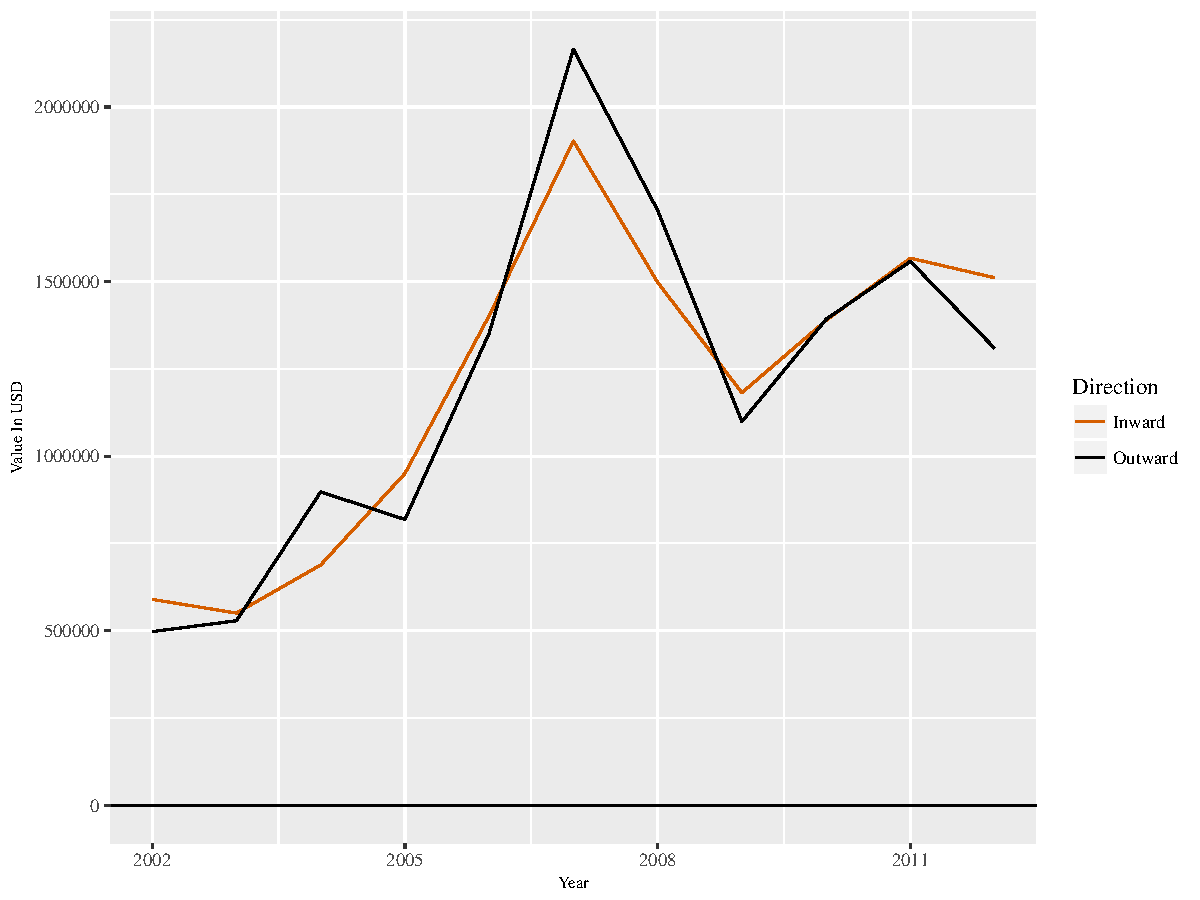
\includegraphics[height=3.5in]{SI_figures/descriptive_plots/fdi_flows.pdf} \vspace{0cm}
%\caption{\label{fig:flows} Global FDI flows by Direction.}
%\end{figure}


\section{Correlations Before and After Rounding FDI} 

In this section we investigate whether the structure of associations between FDI an the dyadic covariates included in the count ERGM is significantly changed by rounding the natural logarithm of FDI

\begin{table}[ht]
\centering
\begin{tabular}{rrrrrrrrrr}
  \hline
 & Lag FDI & GDP prod & Dist & Alliance &Defense& Trade & BIT & Both OECD & PTA \\ 
  \hline
2002 & 0.37 & 0.38 & -0.24 & 0.24 & 0.22 & 0.41 & 0.01 & 0.51 & 0.22 \\ 
  2003 & 0.39 & 0.37 & -0.25 & 0.24 & 0.22 & 0.41 & 0.01 & 0.53 & 0.24 \\ 
  2004 & 0.40 & 0.37 & -0.26 & 0.25 & 0.22 & 0.42 & 0.02 & 0.52 & 0.25 \\ 
  2005 & 0.39 & 0.40 & -0.26 & 0.26 & 0.23 & 0.44 & 0.03 & 0.50 & 0.24 \\ 
  2006 & 0.37 & 0.38 & -0.27 & 0.25 & 0.22 & 0.44 & 0.03 & 0.50 & 0.26 \\ 
  2007 & 0.36 & 0.39 & -0.28 & 0.26 & 0.23 & 0.45 & 0.04 & 0.50 & 0.31 \\ 
  2008 & 0.39 & 0.40 & -0.29 & 0.26 & 0.23 & 0.44 & 0.04 & 0.50 & 0.30 \\ 
  2009 & 0.37 & 0.43 & -0.31 & 0.28 & 0.25 & 0.48 & 0.07 & 0.49 & 0.31 \\ 
  2010 & 0.38 & 0.46 & -0.30 & 0.28 & 0.25 & 0.49 & 0.08 & 0.45 & 0.30 \\ 
  2011 & 0.39 & 0.45 & -0.30 & 0.28 & 0.25 & 0.49 & 0.08 & 0.44 & 0.30 \\ 
  2012 & 0.38 & 0.44 & -0.27 & 0.26 & 0.24 & 0.45 & 0.06 & 0.45 & 0.25 \\ 
   \hline
\end{tabular}
\caption{Correlation between dyadic variables and FDI} \label{tab:cor}
\end{table}

\begin{table}[ht]
\centering
Correlation between dyadic variables and rounded FDI
\begin{tabular}{rrrrrrrrrr}
  \hline
 & Lag FDI & GDP prod & Dist & Alliance &Defense& Trade & BIT & Both OECD & PTA \\ 
  \hline
2002 & 0.36 & 0.38 & -0.24 & 0.24 & 0.21 & 0.40 & 0.01 & 0.51 & 0.22 \\ 
  2003 & 0.39 & 0.37 & -0.25 & 0.24 & 0.22 & 0.41 & 0.01 & 0.52 & 0.24 \\ 
  2004 & 0.40 & 0.37 & -0.26 & 0.25 & 0.22 & 0.42 & 0.02 & 0.52 & 0.25 \\ 
  2005 & 0.39 & 0.39 & -0.26 & 0.26 & 0.23 & 0.44 & 0.03 & 0.50 & 0.24 \\ 
  2006 & 0.36 & 0.38 & -0.27 & 0.25 & 0.22 & 0.44 & 0.03 & 0.50 & 0.26 \\ 
  2007 & 0.36 & 0.39 & -0.28 & 0.26 & 0.23 & 0.44 & 0.04 & 0.50 & 0.30 \\ 
  2008 & 0.38 & 0.40 & -0.29 & 0.25 & 0.23 & 0.44 & 0.04 & 0.50 & 0.30 \\ 
  2009 & 0.36 & 0.43 & -0.31 & 0.28 & 0.25 & 0.47 & 0.07 & 0.49 & 0.31 \\ 
  2010 & 0.37 & 0.46 & -0.30 & 0.28 & 0.25 & 0.49 & 0.08 & 0.45 & 0.30 \\ 
  2011 & 0.39 & 0.44 & -0.29 & 0.28 & 0.25 & 0.48 & 0.08 & 0.44 & 0.30 \\ 
  2012 & 0.38 & 0.44 & -0.26 & 0.26 & 0.24 & 0.45 & 0.06 & 0.44 & 0.25 \\ 
   \hline
\end{tabular}
\caption{Correlation between dyadic variables and FDI} \label{tab:rcor}
\end{table}


\begin{table}[ht]
\centering
Two-tailed $p$-value in test for difference in correlations before and after rounding
\begin{tabular}{rrrrrrrrrr}
  \hline
 & Lag FDI & GDP prod & Dist & Alliance &Defense& Trade & BIT & Both OECD & PTA \\ 
  \hline
2002 & 0.24 & 0.57 & 0.72 & 0.65 & 0.69 & 0.58 & 1.00 & 0.47 & 0.88 \\ 
  2003 & 0.12 & 0.69 & 0.78 & 0.84 & 0.81 & 0.66 & 0.91 & 0.64 & 0.86 \\ 
  2004 & 0.22 & 0.69 & 0.66 & 0.75 & 0.72 & 0.57 & 0.91 & 0.51 & 0.75 \\ 
  2005 & 0.18 & 0.57 & 0.74 & 0.76 & 0.76 & 0.57 & 0.98 & 0.47 & 0.99 \\ 
  2006 & 0.18 & 0.68 & 0.77 & 0.76 & 0.75 & 0.65 & 0.95 & 0.43 & 0.96 \\ 
  2007 & 0.15 & 0.75 & 0.81 & 0.89 & 0.81 & 0.82 & 0.93 & 0.51 & 0.78 \\ 
  2008 & 0.19 & 0.73 & 0.71 & 0.86 & 0.89 & 0.73 & 0.98 & 0.52 & 0.84 \\ 
  2009 & 0.20 & 0.66 & 0.73 & 0.83 & 0.79 & 0.60 & 0.99 & 0.33 & 0.80 \\ 
  2010 & 0.20 & 0.71 & 0.82 & 0.90 & 0.91 & 0.68 & 1.00 & 0.52 & 0.96 \\ 
  2011 & 0.20 & 0.64 & 0.72 & 0.85 & 0.82 & 0.71 & 0.88 & 0.51 & 0.95 \\ 
  2012 & 0.23 & 0.72 & 0.73 & 0.84 & 0.88 & 0.76 & 0.87 & 0.55 & 0.92 \\ 
   \hline
\end{tabular}
\caption{Correlation between dyadic variables and FDI} \label{tab:cortest}
\end{table}



\section{Time-Pooled Model Results}\label{pooledresults}
For robustness checks, we re-estimate the count ERGM by pooling the data, which is common in the literature for regression based models. Figure \ref{fig:net_effects} shows that all network dependence terms are significant in the time-pooled models. Non-OECD pairs exhibit less reciprocity than OECD pairs, but the average effect for the time sample is still positive and significant.

%The exogenous covariates from the pooled model are presented in Table \ref{fig:effectPlots2}.  The results show that ignoring network structure lead to biased estimates in several covariates. We see significant differences in the coefficients for distance, the product of dyad's GDP, the three treaty variables, as well as origin and destination's GDP per capita, Polity, and trade openness. These findings are consistent with those from the yearly models. It illustrates that failure to include network structure results in biased estimates. 



%\begin{landscape}
%\begin{spacing}{.7}
%\begin{longtable}[!h]{c@{\hskip .5cm}c@{\hskip .5cm}c@{\hskip .5cm}c}

%Sum & Sum$^{(1/2)}$ &Non-Zero & Alliance Treaty\\
%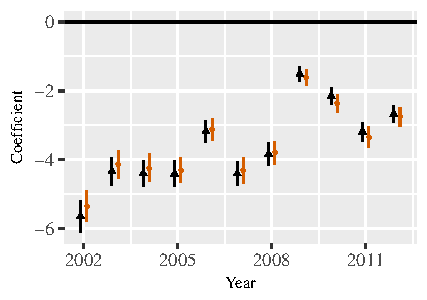
\includegraphics[height=.2\textheight, clip=true, trim=0cm 0cm 0cm .2cm]{SI_figures/plots_pooled/Sum.pdf}    &
%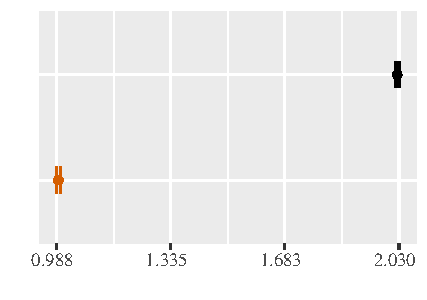
\includegraphics[height=.2\textheight, clip=true, trim=0cm 0cm 0cm .2cm]{SI_figures/plots_pooled/sum_5.pdf}   &
%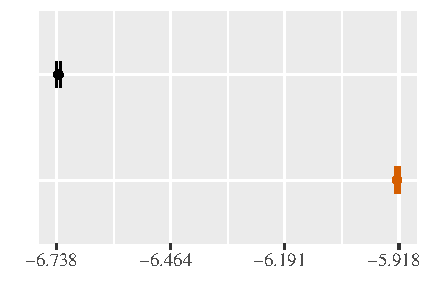
\includegraphics[height=.2\textheight, clip=true, trim=0cm 0cm 0cm .2cm]{SI_figures/plots_pooled/Non-zero.pdf} &
%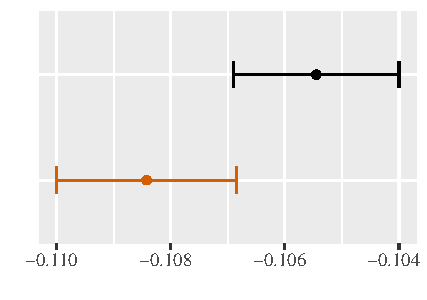
\includegraphics[height=.2\textheight, clip=true, trim=0cm 0cm 0cm .2cm]{SI_figures/plots_pooled/AllianceTreaty.pdf}   \\
%Bilateral Investment Treaty & Defense Treaty &Product of Dyad's GDP & Distance\\
%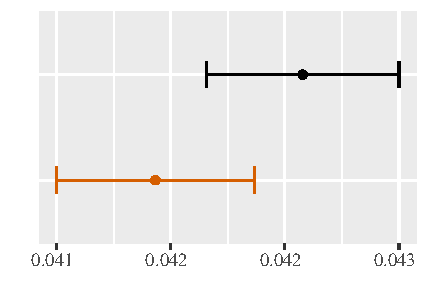
\includegraphics[height=.2\textheight, clip=true, trim=0cm 0cm 0cm .2cm]{SI_figures/plots_pooled/BIT.pdf} &
%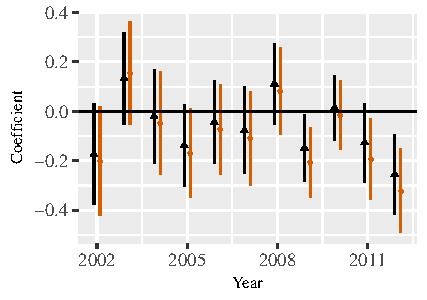
\includegraphics[height=.2\textheight, clip=true, trim=0cm 0cm 0cm .2cm]{SI_figures/plots_pooled/DefenseTreaty.pdf}   &
%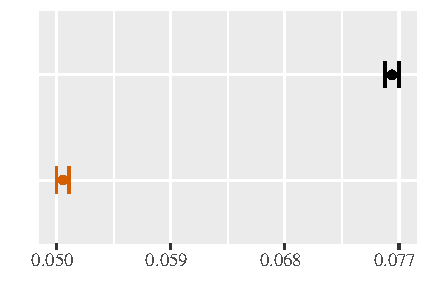
\includegraphics[height=.2\textheight, clip=true, trim=0cm 0cm 0cm .2cm]{SI_figures/plots_pooled/DyadGDPProduct.pdf} &
%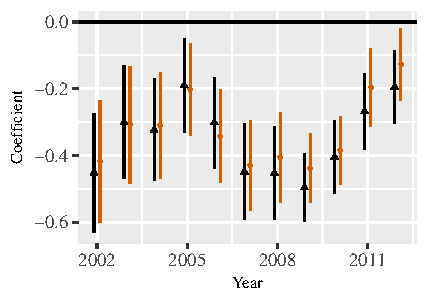
\includegraphics[height=.2\textheight, clip=true, trim=0cm 0cm 0cm .2cm]{SI_figures/plots_pooled/Distance.pdf}   \\
%Lagged FDI stock & Bilateral Trade Volume & GDP per capita, in-degree & GDP per capita, out-degree\\
%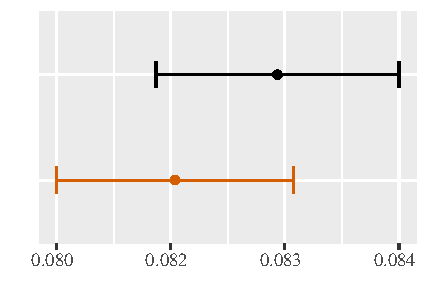
\includegraphics[height=.2\textheight, clip=true, trim=0cm 0cm 0cm .2cm]{SI_figures/plots_pooled/LaggedDV.pdf}    &
%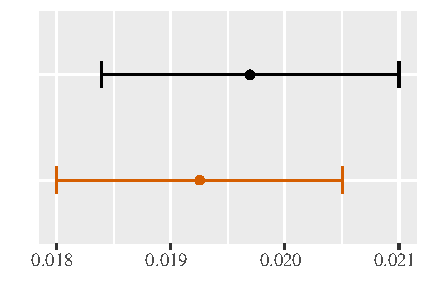
\includegraphics[height=.2\textheight, clip=true, trim=0cm 0cm 0cm .2cm]{SI_figures/plots_pooled/TradeVolume.pdf}   &
%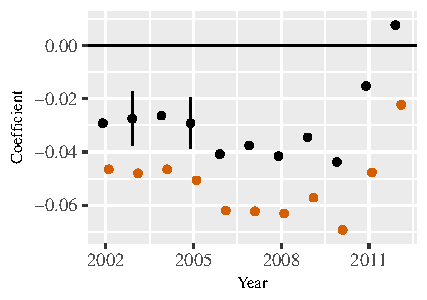
\includegraphics[height=.2\textheight, clip=true, trim=0cm 0cm 0cm .2cm]{SI_figures/plots_pooled/GDPpc_in.pdf} &
%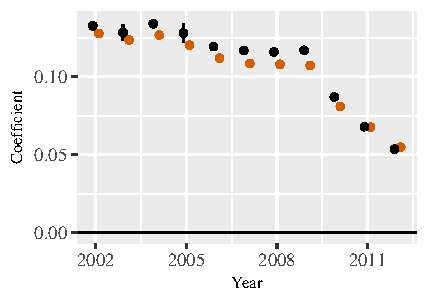
\includegraphics[height=.2\textheight, clip=true, trim=0cm 0cm 0cm .2cm]{SI_figures/plots_pooled/GDPpc_out.pdf}   \\
%Polity, in-degree & Polity, out-degree &Trade Openness, in-degree & Trade Openness, out-degree\\
%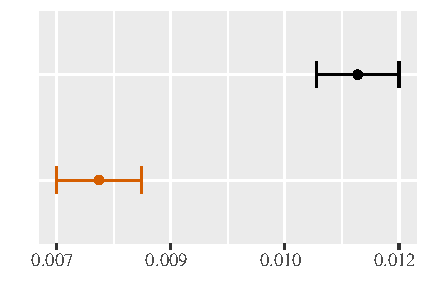
\includegraphics[height=.2\textheight, clip=true, trim=0cm 0cm 0cm .2cm]{SI_figures/plots_pooled/Polity_in.pdf} &
%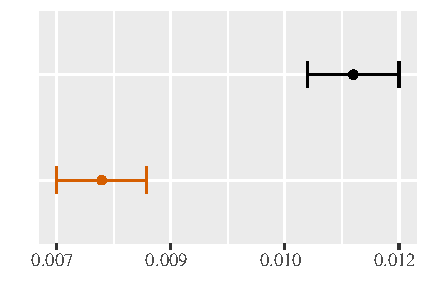
\includegraphics[height=.2\textheight, clip=true, trim=0cm 0cm 0cm .2cm]{SI_figures/plots_pooled/Polity_out.pdf}   &
%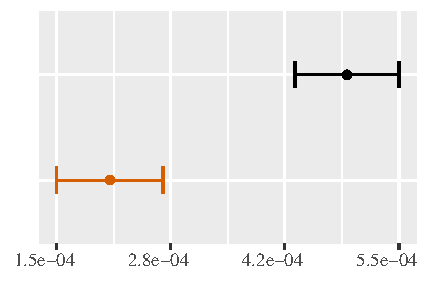
\includegraphics[height=.2\textheight, clip=true, trim=0cm 0cm 0cm .2cm]{SI_figures/plots_pooled/Trade_in.pdf} &
%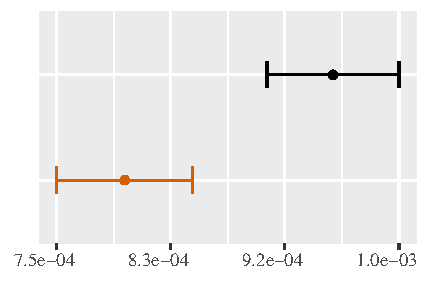
\includegraphics[height=.2\textheight, clip=true, trim=0cm 0cm 0cm .2cm]{SI_figures/plots_pooled/Trade_out.pdf}   \\

%\caption{\label{fig:effectPlots2} Estimates of terms in time-pooled ERGMs. Bars span 95\% confidence intervals. Black coefficient representations are from models excluding dependence terms (i.e., transitivity and reciprocity).}

%\end{longtable}
%\end{spacing}
%\end{landscape}


%Figure \ref{fig:exog_2}  shows that after pooling, network terms remain positive and statistically significant, supporting our hypothesis that reciprocity and transitivity characterize FDI flows. The estimates are similar to yearly results in terms of direction and statistical significance. %As expected from pooling, there are decreases in standard errors because the increased number of observations. %for variables that exhibit more yearly heterogeneity, estimates are on average more different than yearly estimates.


\begin{figure}[htp]
\centering
\begin{tabular}{@{\hskip -.05cm}c@{\hskip .2cm}c@{\hskip .2cm}c}
Transitivity  & Reciprocity, OECD pair &Reciprocity, non-OECD pair\\
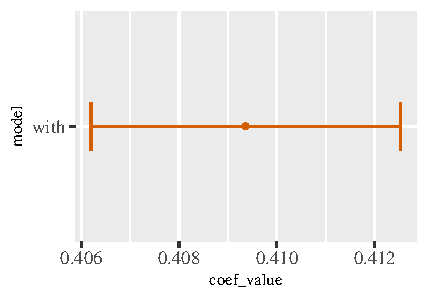
\includegraphics[height=.165\textheight, clip=true, trim=1.3cm .5cm 0cm .1cm]{SI_figures/rl_TERGM_plots/Transitivity.pdf}   &
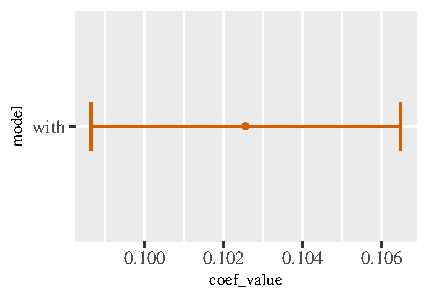
\includegraphics[height=.165\textheight, clip=true, trim=1.3cm .5cm 0cm .1cm]{SI_figures/rl_TERGM_plots/Mutuality_OECD_Pair.pdf}    &
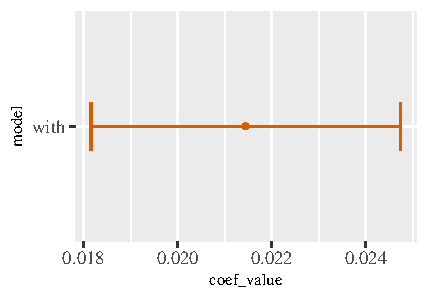
\includegraphics[height=.165\textheight, clip=true, trim=1.3cm .5cm 0cm .1cm]{SI_figures/rl_TERGM_plots/Mutuality_Not_OECD_Pair.pdf} \\
\end{tabular}
\caption{\label{fig:net_effects} Estimates of network terms in time-pooled ERGMs. Bars span 95\% confidence intervals.}
\end{figure}


\section{Latent Space Model Results}\label{LSMresults}


\begin{figure}[!h]
\centering
\begin{tabular}{@{\hskip -.05cm}c@{\hskip .2cm}c}
Transitivity  & Reciprocity\\
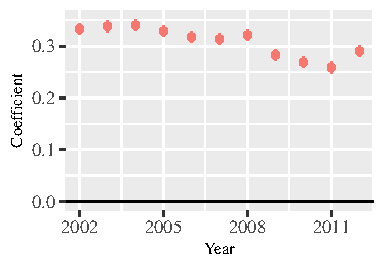
\includegraphics[height=.165\textheight, clip=true, trim=.5cm .5cm 0cm .1cm]{SI_figures/LSM_rl_plots/trans_dep.pdf}   &
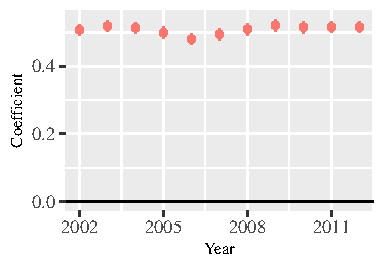
\includegraphics[height=.165\textheight, clip=true, trim=.5cm .5cm 0cm .1cm]{SI_figures/LSM_rl_plots/dyad_dep.pdf} \\
\end{tabular}
\caption{\label{fig:LSMnetterms} Estimates of Dependence terms. Bars span 95\% confidence intervals. }
\end{figure}

\section{Subset by Missingness Results}\label{qlevelresults}

In the paper, we imputed missing values with zeros. In this section, we check whether our results are robust if we analyze a subset of the data set based on the level of missingness. To subset the data, we approximate total level of missingness in the adjacency matrices ({\emph{q}) by using the proportion of missing values for each node (\emph{p}). We conduct two robustness checks: (1) when \emph{p} = 0.86,  \emph{q} $\approx$ 0.50 and  \emph{n} = 70; and (2) when \emph{p} = 0.72, \emph{q} $\approx$ 0.25 and  \emph{n} = 28. In the first case, we only include nodes with missing values that are 86\% or less of the possible edges for the entire data set, which leaves us with an adjacency matrix that is only missing 50\% of the values (70 countries in total). Similarly, the second set only includes nodes with missing values that are 72\% or less of the possible edges for the entire dataset, which leaves us with an adjacency matrix that is only missing 25\% of the values (28 countries in total).  Following our approach in the paper, we impute missing values in the two subsets of the data with zeros.

Figures \ref{fig:q50netterms} and \ref{fig:q25netterms} present the results for the two robustness checks, respectively. We see that FDI networks show strong transitivity for all years, but reciprocity effects become weak and insignificant in some years. This may be because most nodes (i.e. states) in the subsets are developed countries that have substantial two-way FDI flows between them and thus there is little variation in the level of reciprocity.


\subsection{q $\approx$  0.50}

\begin{figure}[!h]
\centering
\begin{tabular}{@{\hskip -.05cm}c@{\hskip .2cm}c@{\hskip .2cm}c}
Transitivity  & Reciprocity, OECD pair &Reciprocity, non-OECD pair\\
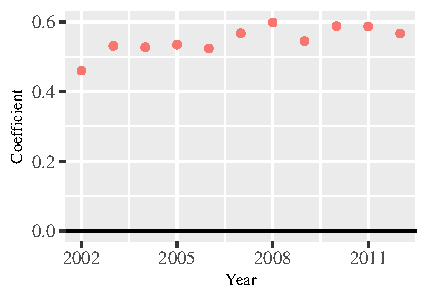
\includegraphics[height=.165\textheight, clip=true, trim=1.3cm .5cm 0cm .1cm]{SI_figures/q50_rl_plots/Transitivity.pdf}   &
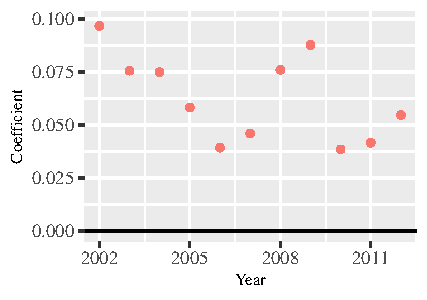
\includegraphics[height=.165\textheight, clip=true, trim=1.3cm .5cm 0cm .1cm]{SI_figures/q50_rl_plots/Mutuality_OECD.pdf}    &
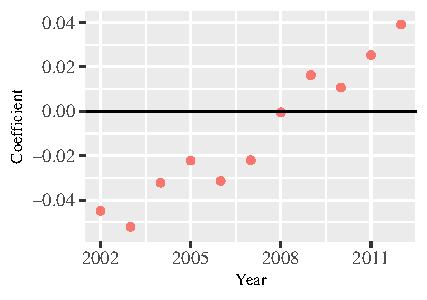
\includegraphics[height=.165\textheight, clip=true, trim=1.3cm .5cm 0cm .1cm]{SI_figures/q50_rl_plots/Mutuality_notOECD.pdf} \\
\end{tabular}
\caption{\label{fig:q50netterms} Estimates of Dependence terms. Bars span 95\% confidence intervals. }
\end{figure}


\subsection{q $\approx$  0.25}

\begin{figure}[!h]
\centering
\begin{tabular}{@{\hskip -.05cm}c@{\hskip .2cm}c@{\hskip .2cm}c}
Transitivity  & Reciprocity, OECD pair &Reciprocity, non-OECD pair\\
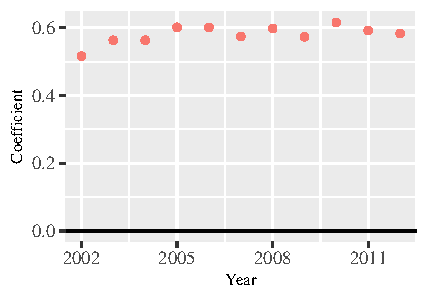
\includegraphics[height=.165\textheight, clip=true, trim=1.3cm .5cm 0cm .1cm]{SI_figures/q25_rl_plots/Transitivity.pdf}   &
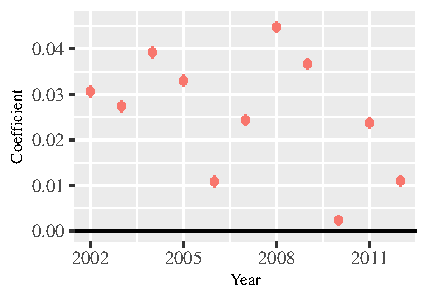
\includegraphics[height=.165\textheight, clip=true, trim=1.3cm .5cm 0cm .1cm]{SI_figures/q25_rl_plots/Mutuality_OECD.pdf}    &
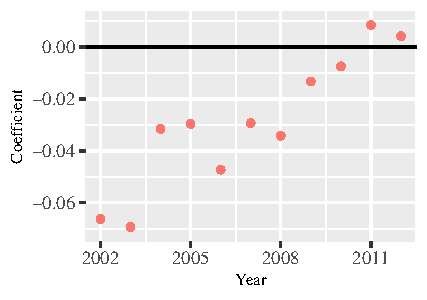
\includegraphics[height=.165\textheight, clip=true, trim=1.3cm .5cm 0cm .1cm]{SI_figures/q25_rl_plots/Mutuality_notOECD.pdf} \\
\end{tabular}
\caption{\label{fig:q25netterms} Estimates of Dependence terms. Bars span 95\% confidence intervals. }
\end{figure}








\section{Tax Incentives and FDI}\label{taxresults}

One potential concern with bilateral FDI data is that they include round-tripping FDI, in which domestic firms transfer funds to a foreign country (typically a tax haven) and invest back as ``foreign capital'' to take advantage of preferential policies that their home countries offer to foreign investors \citep{Borga:2016}. Round-tripping FDI could inflate reciprocity. Further, firms may use tax havens to channel funds to other countries \citep{Borga:2017}. If firms in one country use a tax haven to invest in another country whose firms also invest in the former country, it creates an artificial triangle closure of investment flows (i.e., transitivity). To address these issues in bilateral FDI data and check the robustness of our findings, we re-estimated the model by including the corporate tax rate for both the sending and receiving country\footnote{Corporate tax rate data comes from the World Bank's \emph{World Development Indicators}.} and estimating models that exclude tax havens. The countries dropped as tax havens are Namibia, Trinidad and Tobago, Bahrain, Luxembourg, the United Kingdom, Ireland, and the Netherlands. We used the EU list of 17 countries as a base list, although most of them were not in our sample due to data availability.\footnote{\url{https://ec.europa.eu/taxation_customs/tax-common-eu-list_en}}  We also added Luxembourg, the United Kingdom, Ireland, and the Netherlands since they are often considered cooperative tax havens.\footnote{Matthew C. Klein. ``What the Foreign Direct Investment Data Tell Us About Corporate Tax Avoidance.'' \emph{Financial Times}, November 23, 2017. \url{https://ftalphaville.ft.com/2017/11/23/2196028/what-the-foreign-direct-investment-data-tell-us-about-corporate-tax-avoidance/}} Figure \ref{fig:tax_rates_netterms} plots the results for reciprocity and transitivity for the models with corporate tax rates. We see that the results on reciprocity become a little weaker when tax rates are included, but they remain significant in most years. Including tax rates does not affect transitivity.
Figure \ref{fig:tax_havens_netterms} plots the results for reciprocity and transitivity for the models that exclude tax havens and the results are nearly identical to those with corporate tax rates.

\begin{figure}[!h]
\centering
\begin{tabular}{@{\hskip -.05cm}c@{\hskip .2cm}c@{\hskip .2cm}c}
Transitivity  & Reciprocity, OECD pair &Reciprocity, non-OECD pair\\
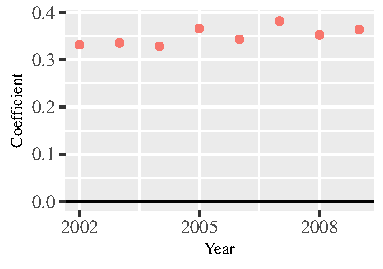
\includegraphics[height=.165\textheight, clip=true, trim=1.3cm .5cm 0cm .1cm]{SI_figures/tax_rl_plots/Transitivity.pdf}   &
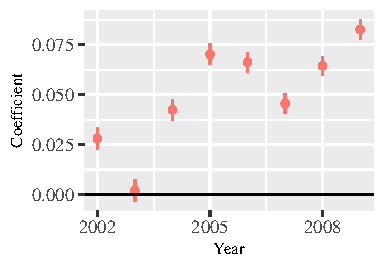
\includegraphics[height=.165\textheight, clip=true, trim=1.3cm .5cm 0cm .1cm]{SI_figures/tax_rl_plots/Mutuality_OECD.pdf}    &
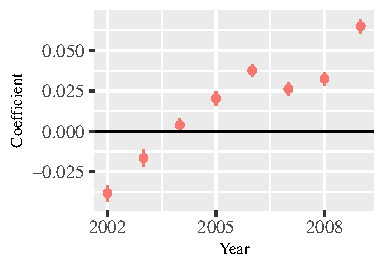
\includegraphics[height=.165\textheight, clip=true, trim=1.3cm .5cm 0cm .1cm]{SI_figures/tax_rl_plots/Mutuality_notOECD.pdf} \\
\end{tabular}
\caption{\label{fig:tax_rates_netterms} Estimates of Dependence terms for models with corporate tax rates. Bars span 95\% confidence intervals. }
\end{figure}

\begin{figure}[!h]
\centering
\begin{tabular}{@{\hskip -.05cm}c@{\hskip .2cm}c@{\hskip .2cm}c}
Transitivity  & Reciprocity, OECD pair &Reciprocity, non-OECD pair\\
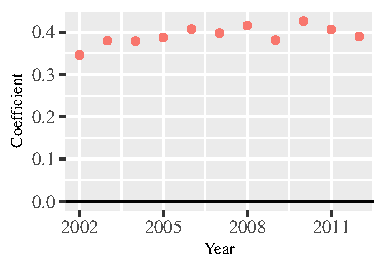
\includegraphics[height=.165\textheight, clip=true, trim=1.3cm .5cm 0cm .1cm]{SI_figures/haven_rl_plots/Transitivity.pdf}   &
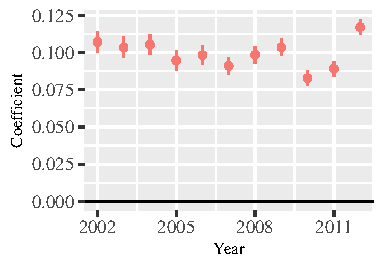
\includegraphics[height=.165\textheight, clip=true, trim=1.3cm .5cm 0cm .1cm]{SI_figures/haven_rl_plots/Mutuality_OECD.pdf}    &
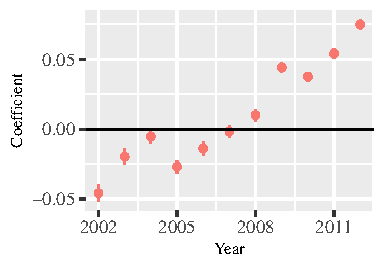
\includegraphics[height=.165\textheight, clip=true, trim=1.3cm .5cm 0cm .1cm]{SI_figures/haven_rl_plots/Mutuality_notOECD.pdf} \\
\end{tabular}
\caption{\label{fig:tax_havens_netterms} Estimates of Dependence terms for models without tax havens. Bars span 95\% confidence intervals. }
\end{figure}


\section{Excluding the European Union}\label{EUresults}

A significant portion of the FDI in the global economy involves the European Union and the majority of the top partners for the EU are other EU countries. This is because of proximity, similar business environments and endowments, and few barriers for EU firms to send FDI to other EU countries. Because of this, there is a high degree of clustering within the EU, and so we run models that drop all EU countries to test if reciprocity and transitivity is still significant for the rest of the global economy. We find that the transitivity statistic remains largely unchanged after dropping EU countries, but that reciprocity is either insignificant or negative for all years except the last two. This supports our point that reciprocity is stronger for Western democracies. However, the positive trend beginning in 2005 indicates that this is changing as FDI between developing countries increases.



\begin{figure}[!h]
\centering
\begin{tabular}{@{\hskip -.05cm}c@{\hskip .2cm}c@{\hskip .2cm}c}
Transitivity  & Reciprocity, OECD pair &Reciprocity, non-OECD pair\\
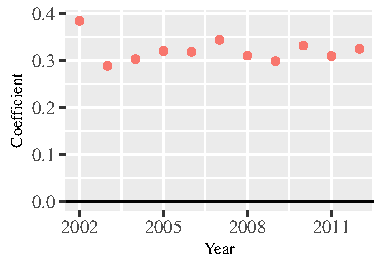
\includegraphics[height=.165\textheight, clip=true, trim=1.3cm .5cm 0cm .1cm]{SI_figures/EU_rl_plots/Transitivity.pdf}   &
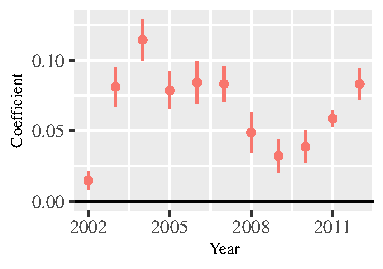
\includegraphics[height=.165\textheight, clip=true, trim=1.3cm .5cm 0cm .1cm]{SI_figures/EU_rl_plots/Mutuality_OECD.pdf}    &
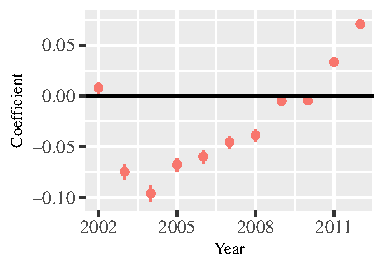
\includegraphics[height=.165\textheight, clip=true, trim=1.3cm .5cm 0cm .1cm]{SI_figures/EU_rl_plots/Mutuality_notOECD.pdf} \\
\end{tabular}
\caption{\label{fig:EU_netterms} Estimates of Dependence terms. Bars span 95\% confidence intervals. }
\end{figure}


\newpage
\singlespacing
\bibliographystyle{apsr}
\bibliography{fdi_reference}






\end{document}


\section{Network Visualizations}\label{visual}

Below are visualizations of the data used in our analysis. In Figure I we see that democratic regimes are more central to the network. This is also evident in Figure J, with more volume of FDI between the US and Europe than elsewhere. We use 2011 as a sample year for the visualizations.

\begin{figure}[!h]
\centering
\includegraphics[scale=.6, clip=true, trim=2cm 2cm 0cm 2.3cm]{SI_figures/visualizations/fdiNet2011.pdf} \vspace{0cm}
\caption{\label{fig:regime_visual} Plot for 2011. Blue to red represents a scale from more autocratic to more democratic regimes.}
\end{figure}

\begin{figure}[!h]
\centering
\includegraphics[scale=.7, clip=true, trim=0cm 9.5cm 0cm 9.5cm]{SI_figures/visualizations/fdi_map.pdf} \vspace{1cm}
\caption{\label{fig:map_visual} Map for 2011. Only includes flows for the 125 countries used in the analysis. Thicker lines represent higher values.}
\end{figure}

Table \ref{tab:describe_binary} provides means for the dichotomous dyadic variables used in our models....

% Table created by stargazer v.5.2 by Marek Hlavac, Harvard University. E-mail: hlavac at fas.harvard.edu
% Date and time: Mon, Feb 20, 2017 - 22:08:59
\begin{table}[htp] \centering
  \caption{}
  \label{}
\begin{tabular}{@{\extracolsep{5pt}}lcccc}
\\[-1.8ex]\hline
\hline \\[-1.8ex]
Statistic &  \multicolumn{1}{c}{Mean} & \multicolumn{1}{c}{St. Dev.} & \multicolumn{1}{c}{Min} & \multicolumn{1}{c}{Max} \\
\hline \\[-1.8ex]
Contiguity &  0.024 & 0.152 & 0 & 1 \\
Common Official Language &  0.112 & 0.315 & 0 & 1 \\
Common Language and Ethnicity &  0.115 & 0.318 & 0 & 1 \\
Former Colonial Relationship &  0.015 & 0.121 & 0 & 1 \\
Common Colonizer &  0.062 & 0.241 & 0 & 1 \\
Defense Treaty &  0.075 & 0.264 & 0 & 1 \\
Non-aggression Treaty &  0.064 & 0.245 & 0 & 1 \\
Neutrality Treaty &  0.004 & 0.063 & 0 & 1 \\
Entente Treaty &  0.066 & 0.248 & 0 & 1 \\
\hline \\[-1.8ex]
\end{tabular}
\caption{\label{tab:describe_binary} Descriptive statistics for dichotomous dyadic covariates. Number of observations across all years is 189,000.}
\end{table}


\includegraphics[scale=.8]{SI_figures/reciprocity.png}\\
\includegraphics[scale=.8]{SI_figures/transitivity.png}\\
\includegraphics[scale=.8]{SI_figures/assortativity.png}\\

\section{Multiple Imputations with Amelia Results}\label{ameliaresults}

In this section, we utilize the \R{} package Amelia to impute the missing values in the full data set,  when \emph{q} $\approx$ 0.50, and when \emph{q} $\approx$ 0.25 \citep{King_et_al:2001,honaker2011amelia}. Figures \ref{fig:full_amelia_netterms} and \ref{fig:q50_amelia_netterms} show the results. We see that transitivity effects are significant in all years and reciprocity effects are also significant in most years. The results in Sections \ref{qlevelresults} and \ref{ameliaresults} give us confidence that our findings regarding the reciprocity and transitivity of FDI are not driven by the pattern of missingness in the data set.

\subsection{Full}

\begin{figure}[!h]
\centering
\begin{tabular}{c@{\hskip 0cm}c}
Reciprocity & Transitivity \\
\includegraphics[height=.2\textheight, clip=true, trim=.5cm .5cm 0cm .2cm]{SI_figures/rl_amelia_full/Mutuality.pdf}    &
\includegraphics[height=.2\textheight, clip=true, trim=.5cm .5cm 0cm .2cm]{SI_figures/rl_amelia_full/Transitivity.pdf}
\end{tabular}
\caption{\label{fig:full_amelia_netterms} Estimates of Dependence terms. Bars span 95\% confidence intervals. }
\end{figure}

\vspace*{-\baselineskip}

\subsection{q $\approx$ 0.50}

\begin{figure}[!h]
\centering
\begin{tabular}{c@{\hskip 0cm}c}
Reciprocity & Transitivity \\
\includegraphics[height=.2\textheight, clip=true, trim=.5cm .5cm 0cm .1cm]{SI_figures/rl_amelia_q50/Mutuality.pdf}    &
\includegraphics[height=.2\textheight, clip=true, trim=.5cm .5cm 0cm .1cm]{SI_figures/rl_amelia_q50/Transitivity.pdf}
\end{tabular}
\caption{\label{fig:q50_amelia_netterms} Estimates of Dependence terms. Bars span 95\% confidence intervals. }
\end{figure}

\clearpage

\subsection{q $\approx$ 0.25}

\begin{figure}[!h]
\centering
\begin{tabular}{c@{\hskip 0cm}c}
Reciprocity & Transitivity \\
\includegraphics[height=.2\textheight, clip=true, trim=.5cm .5cm 0cm .2cm]{SI_figures/rl_amelia_q25/Mutuality.pdf}    &
\includegraphics[height=.2\textheight, clip=true, trim=.5cm .5cm 0cm .2cm]{SI_figures/rl_amelia_q25/Transitivity.pdf}
\end{tabular}
\caption{\label{fig:q25_amelia_netterms} Estimates of Dependence terms. Bars span 95\% confidence intervals. }
\end{figure}

\begin{table}[!htbp] \centering
  \caption{Correlation Matrix}
  \label{}
\begin{tabular}{@{\extracolsep{5pt}} lccccccccc}
\\[-1.8ex]\hline
\hline \\[-1.8ex]
 & Mass & Distance & Polity \\
\hline \\[-1.8ex]
Mass & $1$ & $$-$0.003$ & $0.091$   \\
Distance (logged) & $$-$0.003$ & $1$ & $0.008$  \\
Polity & $0.091$ & $0.008$ & $1$  \\
Trade Openness & $$-$0.166$ & $$-$0.057$ & $$-$0.078$ \\
BITs & $0.141$ & $$-$0.085$ & $0.018$  \\
Trade Volume & $0.714$ & $$-$0.215$ & $0.215$   \\
GDP per capita (logged)& $0.392$ & $$-$0.084$ & $0.166$   \\
Alliance Treaty & $0.133$ & $$-$0.348$ & $0.073$   \\
Defense Treaty & $0.065$ & $$-$0.391$ & $0.065$ \\
\hline \\[-1.8ex]
\\[-1.8ex]\hline
\hline \\[-1.8ex]
 & Trade Openness &BITs &  Trade Volume  \\
\hline \\[-1.8ex]
Mass & $$-$0.166$ & $0.141$& $0.714$  \\
Distance (logged) & $$-$0.057$ & $$-$0.085$ & $$-$0.215$ \\
Polity & $$-$0.078$ & $0.018$& $0.215$  \\
Trade Openness  & $1$ & $0.032$ & $$-$0.055$ \\
BITs & $0.032$ & $1$ & $0.143$ \\
Trade Volume & $$-$0.055$ & $0.143$& $1$  \\
GDP per capita (logged) & $0.225$ & $0.093$ & $0.330$  \\
Alliance Treaty & $$-$0.044$ & $0.021$& $0.216$  \\
Defense Treaty & $$-$0.046$ & $0.010$ & $0.177$   \\
\hline \\[-1.8ex]
\\[-1.8ex]\hline
\hline \\[-1.8ex]
& GDP per capita & Alliance Treaty & Defense Treaty \\
\hline \\[-1.8ex]
Mass & $0.392$ & $0.133$ & $0.065$ \\
Distance & $$-$0.084$ & $$-$0.348$ & $$-$0.391$  \\
Polity & $0.166$ & $0.073$ & $0.065$   \\
Trade Openness & $0.225$ & $$-$0.044$ & $$-$0.046$\\\
BITs & $0.093$ & $0.021$ & $0.010$\\
Trade Volume & $0.330$ & $0.216$ & $0.177$ \\
GDP per capita (logged) & $1$ & $0.098$ & $0.038$ \\
Alliance Treaty & $0.098$ & $1$ & $0.850$ \\
Defense Treaty & $0.038$ & $0.850$ & $1$ \\
\hline \\[-1.8ex]
\end{tabular}
\end{table}

